%
%==> Intro and basic commands
%
\section{Intro and basic commands}

%
%==> Basic commands
%
\begin{frame}[fragile]
  \frametitle{
    Basic commands
  }
  
  \begin{itemize}%[<+->]
  \item
    {\tt git init} - initializes a Git repository.
  \item
    {\tt git add} - adds files to your repository.
  \item
    {\tt git commit} - creates a commit. Commits allow Git to keep track of your revisions, similar to saving files.
  \item
    {\tt git status} - shows the status of your Git repository (i.e. what files have been changed, what files are not accounted for, etc).
  \end{itemize}

\end{frame}

%
%==> The basic git workflow is:
%
\begin{frame}
  \frametitle{
    The basic Git workflow is
  }

  \begin{itemize}%[<+->]
  \item
    \textcolor{blue}{\bf modify files} in your working directory.
  \item
    \textcolor{blue}{\bf stage files} you've worked on. This prepares a snapshot of the directory
  \item
    \textcolor{blue}{\bf commit the files} you've staged. This stores that snapshot in the git repository.
  \end{itemize}

\end{frame}

%
%==> Initializing repositories
%
\begin{frame}[fragile]
  \frametitle{Initializing repositories
  }

  To initialize a new project, in the project directory, initialize the git repository with:

  \begin{lstlisting}
    git init
  \end{lstlisting}

  %Remark: This will enable git to keep track of changes in this folder, and subfolders by creating a {\tt .git} hidden folder containing the git skeleton.

  The second way is:

  \begin{lstlisting}
    git clone https://github.com/jlokimlin
    /intro\_to\_git.git
  \end{lstlisting}

  %Remark: This will clone an existing repository into your currect directory.

  \textcolor{red}{
    {\bf Warning:} Each new repository should be in its own directory. One git repository should {\bf not} be created or cloned in an {\bf existing git repository}, i.e., a folder you've initialized a git repository and its subfolders.
  }

\end{frame}

%
%==> Configuring Git
%
\begin{frame}[fragile]
  \frametitle{
    Configuring Git
  }

  You will have to do this \textcolor{red}{\bf once} per computer you use {\tt git config --global:}

  {
    \footnotesize
    \begin{lstlisting}
      git config --global user.name "Your Avatar"
      git config --global user.email you@domain.com''
      git config --global core.editor vim
      git config color.ui auto
    \end{lstlisting}
  }
  
% Remark: The {\tt --global} option corresponds to a user-wide configuration. The configuration will be stored in a hidden repository in your home. You can also configure each git repository individually, by removing this option, or system-wide by replacing the {\tt --global} option with {\tt --system}. Usually, we just configure repositories user-wide.

  You can check your configuration with:
  \begin{lstlisting}
    git config --list
  \end{lstlisting}

  % Remark: If you've configured git several times at different levels, you will probably see several entries twice or three times in the configuration list. The user-wide configuration overrides the system-wide configuration, and the local configuration overrides the user-wide configuration.

\end{frame}

%
%==> Working locally
%
\begin{frame}[fragile]
  \frametitle{
    Working locally
}

  % Remark: One of the main goal of version control is to save snapshots of your directory. We call those snapshots commits. To each snapshot is associated some metadata: the date the snapshot was taken, who took it, what files where modified, the changes that were made on those files etc. Git will enable you to track the changes made to the files, revert the entire project to a previous snapshot, review changes made over time, view who modified a file. Now that we know why we want to create a snapshot, let's see how to do this.

  Right now, nothing in the project is tracked. First let's create some directories and files in our directory.

  \begin{lstlisting}
    touch README.md
  \end{lstlisting}

  First, you need to tell git this file exists:

  \begin{lstlisting}
    git add README.md
  \end{lstlisting}

  Now you can commit it:

  \begin{lstlisting}
    git commit -m "Added a README file"
  \end{lstlisting}

  At this point, you have one tracked file, and an initial commit. 

\end{frame}

%
%==> File status lifecycle
%
\begin{frame}[fragile]

  % Remark: Each file in the working directory can be in one of two states: tracked or untracked. Any file you have not explicitly added at some point is untracked. Tracked files can themselves be in different states: unmodified, modified or staged.
  
  \begin{center}
    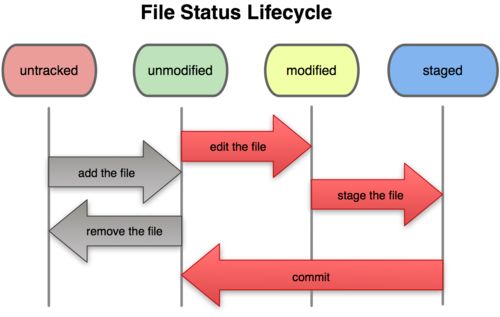
\includegraphics[scale=1.25]{./graphics/git_file_status_lifecycle.png}
  \end{center}

\end{frame}

%
%==> The git status command
%
\begin{frame}[fragile]
  \frametitle{
    The git status command
  }

  The {\tt git status} command will display all untracked files, and modified and staged files in your directory:

  \begin{lstlisting}
    touch AUTHORS.txt
    git status
  \end{lstlisting}

  Now, try
  \begin{lstlisting}
    git add AUTHORS.txt
    git status
  \end{lstlisting}

  {\tt git add} is also used to stage file. In fact, running {\tt git add} on an untracked file not only tracks it, but stages it.

  \begin{lstlisting}
    git commit -m "Added the AUTHORS file"
  \end{lstlisting}

  And here is the second commit! 

\end{frame}
%
%==> Tracking changes to a modified file
%
\begin{frame}[fragile]
  \frametitle{
    Tracking changes to a modified file
  }

  Sometimes, you may want to look at the changes you've made to a modified file:

  \begin{lstlisting}
    git diff
  \end{lstlisting}

  To look at the changes you've made in the staged files, simply use:

  \begin{lstlisting}
    git diff --cached
  \end{lstlisting}

  And to view the history of all commits:

  \begin{lstlisting}
    git log
  \end{lstlisting}

\end{frame}

%
%==> (Re)moving files
%
\begin{frame}[fragile]
  \frametitle{
    (Re)moving files
  }

  \begin{itemize}
  \item
    \textcolor{red}{Deleting files:} Why use {\tt git rm} to remove a file instead of {\tt rm}?
    \begin{itemize}
    \item
      If you just use {\tt rm}, you will need to follow it up with {\tt git add <fileRemoved>} The command {\tt  git rm} does both in one step.
    \item
      You can also use {\tt git rm --cached} which will remove the file from the index (staging it for deletion on the next commit), but keep your copy in the local file system.
      \end{itemize}
  \item
    \textcolor{red}{Moving files:} In a similar fashion, {\tt git mv} can be used to move a file in one step.
  \end{itemize}

\end{frame}

%
%==> Canceling stages
%
\begin{frame}[fragile]
  \frametitle{
    Canceling stages
  }
  
  %Remark: Because to err is human, you may want to cancel some stages.
  Two scenarios may occur:
  \begin{enumerate}
  \item
    \textcolor{blue}{you staged a file you do not want to commit}
  \item
    \textcolor{red}{you made some changes on a file you want to cancel.}
  \end{enumerate}

  First, let's assume you've staged a file you want to unstage:

  \begin{lstlisting}
    touch myFile.tex
    git add myFile.tex
  \end{lstlisting}

  To unstage it, run:

  \begin{lstlisting}
    git reset HEAD myFile.tex
  \end{lstlisting}

  %Remark: The syntax is git reset HEAD <filename>. We will explain what HEAD is later on.
  Second, say you've modified a file and you want to cancel the changes.
  \begin{lstlisting}
    git checkout myFile.tex
  \end{lstlisting}

  %Remark: If you run {\tt git status}, you can notice git reminds you what command to use for which action.
  
\end{frame}
